\documentclass{article}
\usepackage{amssymb}
\usepackage{xstring}
\usepackage{amsmath}
\usepackage{verbatim}
\usepackage{graphicx}
\usepackage{listings}
\usepackage{color} \usepackage{transparent}
\let\oldsum\sum
\renewcommand{\sum}{\oldsum\limits}

\newcommand{\mboldescrip}[5]{
\vspace{0.5in}
    \textbf{#1}:
    \begin{itemize}
        \item Latex: #2
        \item Mathematical notation: #3
        \item Description: #4
        \item Example: #5
    \end{itemize}
}

\begin{document}

\title{Math-Based Optimization Language (MBOL)}

\author{Andrew Newell}

\maketitle

\tableofcontents

\section{Introduction}

This document should explain the MBOL language which is a subset of the Latex language. The goal is to convert natural mathematical representations of optimization programs into a solver. Currently MBOL supports linear programs or mixed integer programs.

\begin{figure}
    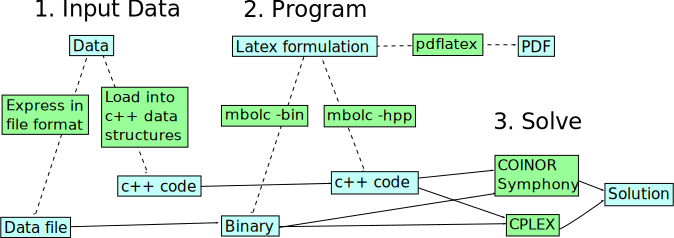
\includegraphics[width=\textwidth]{figures/mbol-overview.pdf}
    \caption{Overview of workflow using MBOL}
    \label{lab:overview}
\end{figure}

Figure~\ref{lab:overview} shows an overview of the problem

\section{Getting Started}

The best flow to get started is to compile the code, setup your environment, and try out the sample programs.

\subsection{Compiling}

\textbf{Requirements}: yacc, lex, and g++ which are all common utilities especially for compiling compilers.

\textbf{Compile}: Execute ``make'' in the top-level directory. The resulting binary ``mbolc'' (MBOL compiler), will be in the ``bin'' directory.

\textbf{Install}: Execute ``sudo make install'' if you would like ``mbolc'' to be added to /usr/bin.

\subsection{Environment setup}

The MBOL compiler creates code that requires files in the include directory. In the top-level directory execute the following:
\begin{verbatim}
export MBOL_HOME=`pwd`
\end{verbatim}
You may want to add some equivalent of this in your ``.bashrc''.

Currently, we support solving with CPLEX through their Concert API or any other solver that can read the mixed integer program format ``.mps''. To solve with CPLEX through Concert, you must setup the CPLEX\_HOME environment variable to point to CPLEX's home directory. For other solvers, e.g. ``symphony'', you need to ensure the executable that solves a given ``.mps'' is available to be invoked.

\subsection{Sample programs}

Sample programs are provided in the ``samples'' directory. Type ``make'' to create code, ``./main'' to try running the code, and ``make svm'' to create some visuals based on the SVM part of the sample code. 

After compiling, notice that the pdf directory contains the pdf versions of each mbol-source file. By understanding how things were built here, much of mbolc can be understood to see how to create code, pdfs, and binaries. 

A binary is created in the maxflow directory for one particular problem. The binary requires no c++ code for data input, but it requires a special input file format shown in this maxflow directory.

\section{MBOL Language}

The language for MBOL is a subset of the Latex language. Latex is the standard for nearly any commonly used mathematical notation. MBOL is a subset of mathematical notation which is already commonly used to describe optimization problems. By specifying this strict subset of the language, MBOL syntax can be compiled into an optimization program that can be used by various state-of-the-art solvers.

The goal here is to describe the details of the grammar of the language. The full grammar is included in this directory under mbol-grammar.txt which is comprehensive as it is automatically generated, but this full grammar does not explain how the grammar affects the optimization programs.

\subsection{Grammar}


\subsection{Operators}

\mboldescrip{Strict subset}{X \textbackslash subset Y}{$X \subset Y$}{Creates all possible subsets for summations or constraints}{$Y=\{1,2,3\}$ implies that we get the following 7 sets $X=\{\},\{1\},\{2\},\{3\},\{1,2\},\{1,3\},\{2,3\}$}

\mboldescrip{Subset}{X \textbackslash subseteq Y}{$X \subseteq Y$}{Creates all possible subsets for summations or constraints}{$Y=\{1,2,3\}$ implies that we get the following 8 sets $X=\{\},\{1\},\{2\},\{3\},\{1,2\},\{1,3\},\{2,3\},\{1,2,3\}$}

\mboldescrip{Integer constraint}{x \textbackslash in \textbackslash mathbb\{Z\}}{$x\in \mathbb{Z}$}{Variable $x$ is constrained to be an integer variable}{$x \in \mathbb{Z}$ implies $x = ...,-2,-1,0,+1,+2,...$}

\mboldescrip{Comparison operators}{= $<$ $>$ \textbackslash le \textbackslash ge}{$= < > \le \ge$}{Constraint operatorst which could constrain the program or even a constraint placed on variables of a summation or constraint set}{Standard equality/inequality operators}

\mboldescrip{Tuple}{(i, j, k)}{$(i,j,k)$}{Tuple of elements, where each element could be a set, tuple, or integer}{$(i,j,k)$ is a 3-tuple, where $i$ could be a set $i=\{1,2\}$, $j$ could be another tuple with two integers $j=(5,7)$, and $k$ could be a simple integer $k=2$}

\mboldescrip{Emptyset}{\textbackslash emptyset}{$\emptyset$}{Set with no elements, useful for putting conditions on whether certain constraints or iterations of a summation are used}{$\emptyset \ne S$ implies that $S$ cannot be empty}

\mboldescrip{Counting iteration}{x=a,...,b}{$x=a,...,b$}{Iterates from integers $a$ to $b$ counting by 1}{$x=a,...,b$ where $a=2$ and $b=8$ will result in $x=2,3,4,5,6,7,8$}

\mboldescrip{Inequality iteration}{a \textbackslash le x \textbackslash le b}{$a \le x \le b$}{Iterates from integers $a$ to $b$ counting by 1}{$a \le x \le b$ where $a=2$ and $b=8$ will result in $x=2,3,4,5,6,7,8$}

\mboldescrip{Set minus}{X \textbackslash setminus Y}{$X \setminus Y$}{Removes elements of $Y$ from $X$}{$\{1,2,5,6,7\} \setminus \{2,3,4,5\} = \{1,6,7\}$}

\mboldescrip{Set union}{X \textbackslash cup Y}{$X \cup Y$}{Creates the union of sets $Y$ and $X$}{$\{1,2,5,6,7\} \cup \{2,3,4,5\} = \{1,2,3,4,5,6,7\}$}

\mboldescrip{Set intersect}{X \textbackslash cap Y}{$X \cap Y$}{Creates the intersect of sets $Y$ and $X$}{$\{1,2,5,6,7\} \cap \{2,3,4,5\} = \{2,5\}$}

\mboldescrip{Set creator}{\{x : x \textbackslash in Y, x $>$ 5\}}{$\{x : x \in Y, x > 5\}$}{Creates a set with specified qualifiers}{$\{x : x \in \{1,4,5,6,8,9\}, x > 5\}=\{6,8,9\}$}

\mboldescrip{Set}{\{x, y, z\}}{$\{x,y,z\}$}{Creates a set with the elements listed}{$\{x,y,z\}$ is a set of these 3 elements}

\mboldescrip{Cardinality}{$|$ X $|$}{$|X|$}{The number of elements in the set}{$|\{6,7,9\}| = 3$}

\mboldescrip{Exponent}{(x)\^{}\{y\}}{$(x)^{y}$}{Raise a value $x$ to the power $y$}{$(2)^{3}=8$}

\mboldescrip{Fraction}{\textbackslash frac\{x\}\{y\}}{$\frac{x}{y}$}{$x$ divided by $y$}{$\frac{9}{4}=2.25$}

\mboldescrip{Indices}{x\_\{i,j\}}{$x_{i,j}$}{$(i,j)th$ value of $x$}{$x_{i,j}$ could stand for the $i$th row and $j$th column of a matrix}

\mboldescrip{Set summation}{\textbackslash sum\_\{a \textbackslash in S \}(x\_a)}{$\sum_{a \in S}(x_a)$}{Sum all values $x_a$ where $a$ is in $S$}{$\sum_{a \in \{1,5,6,7\}}(x_a) = x_1+x_5+x_6+x_7$}

\mboldescrip{Counting summation}{\textbackslash sum\_\{i = 1\}\^{}\{n\}(x\_i)}{$\sum_{i=1}^{n}(x_i)$}{Sum all values $x_i$ where $1 \le i \le n$}{$\sum_{i=1}^{5}(x_i) = x_1+x_2+x_3+x_4+x_5$}

\end{document}
